\documentclass[../main.tex]{subfiles}
\graphicspath{{\subfix{../images/}}}
\begin{document}

\begin{figure}[htb!]
\centering
  
\includegraphics[width=7cm]{fat-foods}
  \caption{Foods rich in fats~\cite{FatFoods}}
\end{figure}

Fats are the most important fuels for the human body, next to carbohydrates.\index{fat}
They have about 9 kcal (37 kJ) per gram (255 kJ/ 1050 kJ per oz), a bit more than double the energy content than carbohydrates and fats.
Fats also have a big signification as building blocks for cells and organs.
The brain for instance consists of 50\% of fat, the white brain matter even 70\%.
But fats are also very important when it's about protecting the organism,
either as insulation against heat and cold or as a cushion for organs and the nervous system.
One of the main constituents of fats are the fatty acids\index{fatty acid}.
One part of these fatty acids, like for instance omega--3 and omega--6 fatty acids\index{fatty acid!omega--3}\index{fatty acid!omega--6}
can't be build by the human body, therefor they are essential to us.
Fatty acids are contained in both, in plant based and animal based foods.

Fats or lipids have the following characteristics:
\begin{itemize}
\item important fuel for our cells, as body fat also as an energy reserve
\item as body fat, it protects the organism of heat and cold, and the organs and nervous system of mechanical shocks
\item they are carrier of the fat--soluble vitamins A, D, E and K\index{vitamin!fat--soluble}
\item in foods, fats are popular as carriers of taste. On top of that
  they cause a good feeling of saturation and prolong the passage of the foods through the colon
\item fats are an important ingredient for the cell membranes\index{cell membranes}
\item certain fats are contributing to the mechanisms of the immune system\index{immune system}
\item they are the building blocks for hormones and vitamins\index{hormones} 
\end{itemize}

\subsection{Structure of Fats}

In nutrition, fats appear in solid form as fats or in liquid form as oils.
Nutritional fats (triglycerides)\index{triglycerides} are compounds consisting of glycerol and three fatty acids, each.
For the fatty acids, we distinguish  between saturated,
monounsaturated and polyunsaturated fatty acids.\index{fatty acid!saturated}\index{fatty acid!unsaturated}

\vspace{3mm}
{\centering
  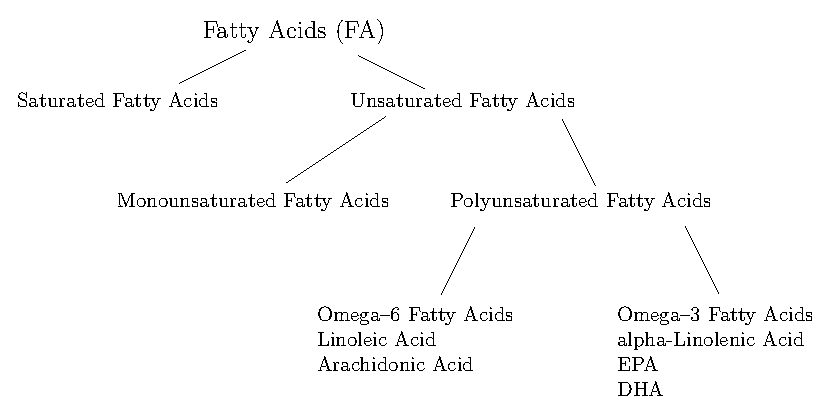
\includegraphics[width=11cm]{FattyAcids}
}

\begin{description}
\item[Saturated Fatty Acids] can be build up by human body.
  Certain saturated fatty acids increase the concentration of cholesterol\index{cholesterol} in the blood.
\item[Some Polyunsaturated Fatty Acids] can't be build up by our body and are therefore essential\index{fatty acid!essential}.
  Among those are omega--6 fatty acids\index{fatty acid!omega--6} linoleic acid\index{fatty acid!linoleic} and the
  omega--3 fatty acids\index{fatty acid!omega--3} alpha--linolenic acid\index{fatty acid!alpha--linolenic} and its derivatives
  eicosapentaenoic acid (EPA)\index{EPA} and docosahexaenoic acid (DHA).\index{DHA}
  Contrary to saturated fatty acids, polyunsaturated fatty acids can lower the cholesterol levels in the blood.
\end{description}

\begin{table}[htb!]
  \centering
  \begin{tabular}{l|ll}
    \textbf{Fatty Acid} & \multicolumn{2}{c}{\textbf{Foods}} \\
                        & \textbf{animal base} & \textbf{plant based} \\
    \hline
    Saturated & meat, sausage, cheese, cream & cocoa and palm oils, \\
                        & lard, shortening, suet \\
    Monounsaturated & goose fat, eggs & olive, canola, and soy oils, \\
                        & & nuts, avocado \\
    Polyunsaturated & \multicolumn{2}{c}{\textit{Omega--3:}} \\
                        & fatty ocean fish (herring,  & linen, soy , hemp and \\
                        & salmon, mackerel), anchovy & walnut oil, walnuts ,algae,\\
                        & sardine, venison & leavy greens \\
  & \multicolumn{2}{c}{\textit{Omega--6:}} \\  
                        & meat, butter, milk and & sunflower, thistle, \\
                        & milk products & pumkin seed, corn seed and \\
                        & & grape seed oils \\

  \end{tabular}
  \caption{Foods and the fatty acids they contain}
\end{table}


\end{document}